\section{\it Range sum queries}

\begin{frame}[fragile]{\textit{Range sum query} em uma árvore de Fenwick}

    \begin{itemize}
        \item Considere que 
        \[
            [1, j] = I_{k_1} \cup I_{k_2} \cup \ldots I_{k_r},
        \]
        com $r = O(\log N)$, $I_a \cap I_b = \emptyset$ se $a\neq b$ e $I_k$ é o intervalo associado
        a $t_k$

        \item Por exemplo,
        \[
            [1, 15] = [1, 8]\cup [9, 12]\cup [13, 14]\cup [15, 15]
        \]

        \item Defina
        \[
            S(j) = \sum_{i = k_1}^{k_r} t_i
        \]

        \item Assim, fazendo $t_0 = 0$, segue que
        \[
            RSQ(i, j) = S(j) - S(i - 1)
        \]

    \end{itemize}

\end{frame}

\begin{frame}[fragile]{Identificação da decomposição de intervalos}

    \begin{itemize}
        \item Para encontrar a decomposição de um intervalo $[1, j]$ em intervalos disjuntos 
            associados aos elementos $t_k$, é preciso computar os valores de $p(n)$

        \item De fato, $p(n)$ corresponde ao \textit{bit} menos significativo de $n$ em base
            binária

        \item Este \textit{bit} pode ser determinado de forma eficiente através de uma operação
            binária
        \[
            p(n) = n \land (-n),
        \]
        onde $\land$ corresponde ao \lq\lq e\rq\rq\ lógico

        \item Os índices $r_i$ dos intervalos $I$ que decompõem $[1,j]$ formam a sequência
            de inteiros positivos 
        \[
            j, j - p(j), [j - p(j)] - p(j - p(j)), \ldots,
        \]
    \end{itemize}

\end{frame}

\begin{frame}[fragile]{Implementação da RSQ em uma BITree}
    \inputsnippet{cpp}{14}{33}{codes/ft.cpp}
\end{frame}

\begin{frame}[fragile]{Visualização de uma RSQ em uma BITree}

    \begin{figure}
        \centering

        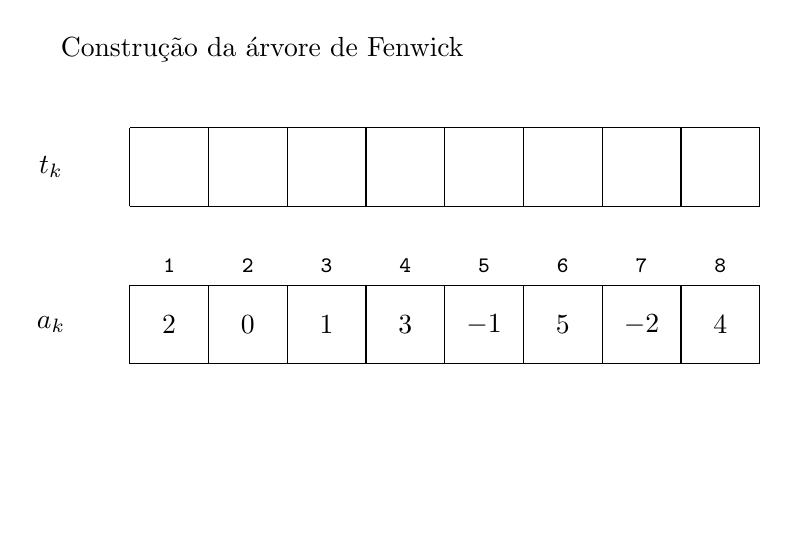
\begin{tikzpicture}
            \node[anchor=west] at (0, 12) { Construção da árvore de Fenwick };

            \draw (1, 10) grid (9, 11);
            \draw (1, 8) grid (9, 9);

            \node at (0, 8.5) { $a_k$ };
            \node at (0, 10.5) { $t_k$ };

            \node[opacity=0, anchor=west] at (0, 6.5) { $RSQ(3,7) = RSQ(1, 7) - RSQ(1, 2)$ };

            \node at (1.5, 9.25) { \footnotesize \tt 1 };
            \node at (2.5, 9.25) { \footnotesize \tt 2 };
            \node at (3.5, 9.25) { \footnotesize \tt 3 };
            \node at (4.5, 9.25) { \footnotesize \tt 4 };
            \node at (5.5, 9.25) { \footnotesize \tt 5 };
            \node at (6.5, 9.25) { \footnotesize \tt 6 };
            \node at (7.5, 9.25) { \footnotesize \tt 7 };
            \node at (8.5, 9.25) { \footnotesize \tt 8 };

            \node at (1.5, 8.5) { $2$ };
            \node at (2.5, 8.5) { $0$ };
            \node at (3.5, 8.5) { $1$ };
            \node at (4.5, 8.5) { $3$ };
            \node at (5.5, 8.5) { $-1$ };
            \node at (6.5, 8.5) { $5$ };
            \node at (7.5, 8.5) { $-2$ };
            \node at (8.5, 8.5) { $4$ };

        \end{tikzpicture}

    \end{figure}

\end{frame}

\begin{frame}[fragile]{Visualização de uma RSQ em uma BITree}

    \begin{figure}
        \centering

        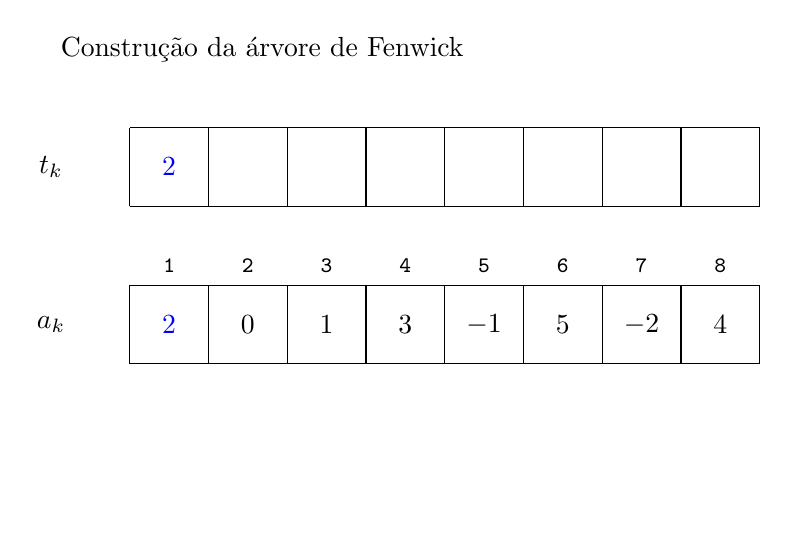
\begin{tikzpicture}
            \node[anchor=west] at (0, 12) { Construção da árvore de Fenwick };

            \draw (1, 10) grid (9, 11);
            \draw (1, 8) grid (9, 9);

            \node at (0, 8.5) { $a_k$ };
            \node at (0, 10.5) { $t_k$ };

            \node[opacity=0, anchor=west] at (0, 6.5) { $RSQ(3,7) = RSQ(1, 7) - RSQ(1, 2)$ };

            \node at (1.5, 9.25) { \footnotesize \tt 1 };
            \node at (2.5, 9.25) { \footnotesize \tt 2 };
            \node at (3.5, 9.25) { \footnotesize \tt 3 };
            \node at (4.5, 9.25) { \footnotesize \tt 4 };
            \node at (5.5, 9.25) { \footnotesize \tt 5 };
            \node at (6.5, 9.25) { \footnotesize \tt 6 };
            \node at (7.5, 9.25) { \footnotesize \tt 7 };
            \node at (8.5, 9.25) { \footnotesize \tt 8 };

            \node at (1.5, 8.5) { \textcolor{blue}{$2$} };
            \node at (2.5, 8.5) { $0$ };
            \node at (3.5, 8.5) { $1$ };
            \node at (4.5, 8.5) { $3$ };
            \node at (5.5, 8.5) { $-1$ };
            \node at (6.5, 8.5) { $5$ };
            \node at (7.5, 8.5) { $-2$ };
            \node at (8.5, 8.5) { $4$ };

            \node at (1.5, 10.5) { \textcolor{blue}{$2$} };
        \end{tikzpicture}

    \end{figure}

\end{frame}

\begin{frame}[fragile]{Visualização de uma RSQ em uma BITree}

    \begin{figure}
        \centering

        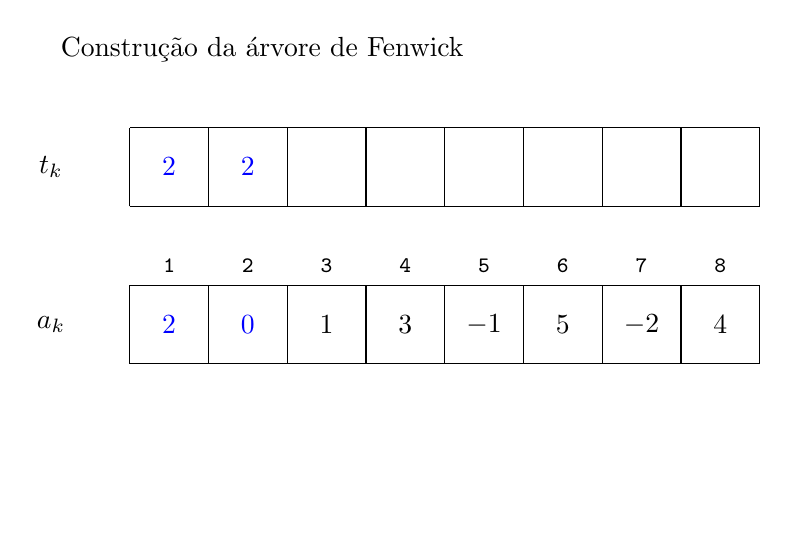
\begin{tikzpicture}
            \node[anchor=west] at (0, 12) { Construção da árvore de Fenwick };

            \draw (1, 10) grid (9, 11);
            \draw (1, 8) grid (9, 9);

            \node at (0, 8.5) { $a_k$ };
            \node at (0, 10.5) { $t_k$ };

            \node[opacity=0, anchor=west] at (0, 6.5) { $RSQ(3,7) = RSQ(1, 7) - RSQ(1, 2)$ };

            \node at (1.5, 9.25) { \footnotesize \tt 1 };
            \node at (2.5, 9.25) { \footnotesize \tt 2 };
            \node at (3.5, 9.25) { \footnotesize \tt 3 };
            \node at (4.5, 9.25) { \footnotesize \tt 4 };
            \node at (5.5, 9.25) { \footnotesize \tt 5 };
            \node at (6.5, 9.25) { \footnotesize \tt 6 };
            \node at (7.5, 9.25) { \footnotesize \tt 7 };
            \node at (8.5, 9.25) { \footnotesize \tt 8 };

            \node at (1.5, 8.5) { \textcolor{blue}{$2$} };
            \node at (2.5, 8.5) { \textcolor{blue}{$0$} };
            \node at (3.5, 8.5) { $1$ };
            \node at (4.5, 8.5) { $3$ };
            \node at (5.5, 8.5) { $-1$ };
            \node at (6.5, 8.5) { $5$ };
            \node at (7.5, 8.5) { $-2$ };
            \node at (8.5, 8.5) { $4$ };

            \node at (1.5, 10.5) { \textcolor{blue}{$2$} };
            \node at (2.5, 10.5) { \textcolor{blue}{$2$} };

        \end{tikzpicture}

    \end{figure}

\end{frame}

\begin{frame}[fragile]{Visualização de uma RSQ em uma BITree}

    \begin{figure}
        \centering

        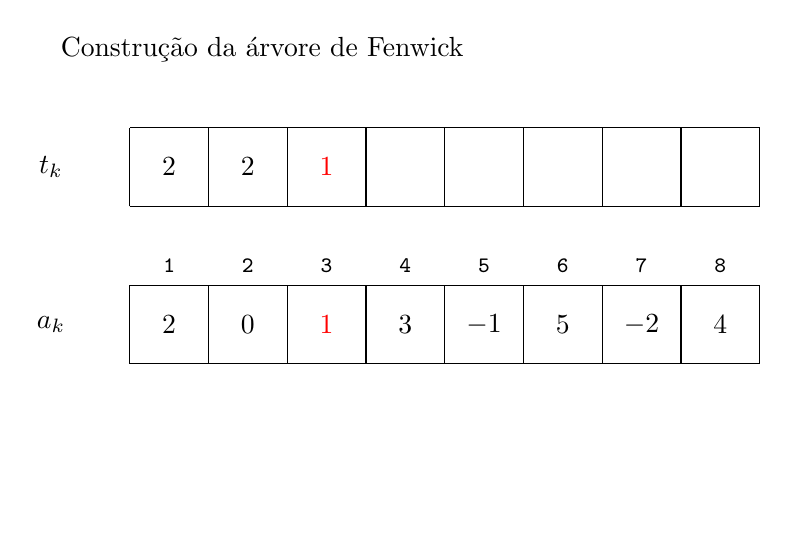
\begin{tikzpicture}
            \node[anchor=west] at (0, 12) { Construção da árvore de Fenwick };

            \draw (1, 10) grid (9, 11);
            \draw (1, 8) grid (9, 9);

            \node at (0, 8.5) { $a_k$ };
            \node at (0, 10.5) { $t_k$ };

            \node[opacity=0, anchor=west] at (0, 6.5) { $RSQ(3,7) = RSQ(1, 7) - RSQ(1, 2)$ };

            \node at (1.5, 9.25) { \footnotesize \tt 1 };
            \node at (2.5, 9.25) { \footnotesize \tt 2 };
            \node at (3.5, 9.25) { \footnotesize \tt 3 };
            \node at (4.5, 9.25) { \footnotesize \tt 4 };
            \node at (5.5, 9.25) { \footnotesize \tt 5 };
            \node at (6.5, 9.25) { \footnotesize \tt 6 };
            \node at (7.5, 9.25) { \footnotesize \tt 7 };
            \node at (8.5, 9.25) { \footnotesize \tt 8 };

            \node at (1.5, 8.5) { \textcolor{black}{$2$} };
            \node at (2.5, 8.5) { \textcolor{black}{$0$} };
            \node at (3.5, 8.5) { \textcolor{red}{$1$} };
            \node at (4.5, 8.5) { $3$ };
            \node at (5.5, 8.5) { $-1$ };
            \node at (6.5, 8.5) { $5$ };
            \node at (7.5, 8.5) { $-2$ };
            \node at (8.5, 8.5) { $4$ };

            \node at (1.5, 10.5) { \textcolor{black}{$2$} };
            \node at (2.5, 10.5) { \textcolor{black}{$2$} };
            \node at (3.5, 10.5) { \textcolor{red}{$1$} };

        \end{tikzpicture}

    \end{figure}

\end{frame}

\begin{frame}[fragile]{Visualização de uma RSQ em uma BITree}

    \begin{figure}
        \centering

        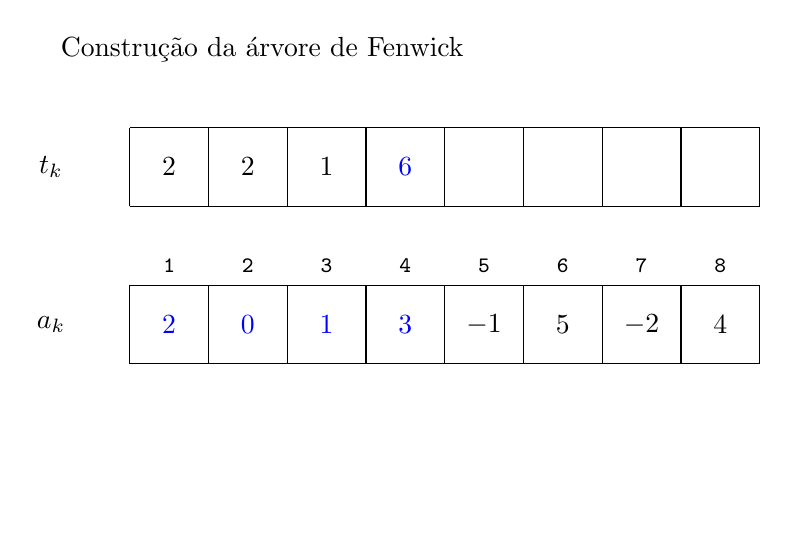
\begin{tikzpicture}
            \node[anchor=west] at (0, 12) { Construção da árvore de Fenwick };

            \draw (1, 10) grid (9, 11);
            \draw (1, 8) grid (9, 9);

            \node at (0, 8.5) { $a_k$ };
            \node at (0, 10.5) { $t_k$ };

            \node[opacity=0, anchor=west] at (0, 6.5) { $RSQ(3,7) = RSQ(1, 7) - RSQ(1, 2)$ };

            \node at (1.5, 9.25) { \footnotesize \tt 1 };
            \node at (2.5, 9.25) { \footnotesize \tt 2 };
            \node at (3.5, 9.25) { \footnotesize \tt 3 };
            \node at (4.5, 9.25) { \footnotesize \tt 4 };
            \node at (5.5, 9.25) { \footnotesize \tt 5 };
            \node at (6.5, 9.25) { \footnotesize \tt 6 };
            \node at (7.5, 9.25) { \footnotesize \tt 7 };
            \node at (8.5, 9.25) { \footnotesize \tt 8 };

            \node at (1.5, 8.5) { \textcolor{blue}{$2$} };
            \node at (2.5, 8.5) { \textcolor{blue}{$0$} };
            \node at (3.5, 8.5) { \textcolor{blue}{$1$} };
            \node at (4.5, 8.5) { \textcolor{blue}{$3$} };
            \node at (5.5, 8.5) { $-1$ };
            \node at (6.5, 8.5) { $5$ };
            \node at (7.5, 8.5) { $-2$ };
            \node at (8.5, 8.5) { $4$ };

            \node at (1.5, 10.5) { \textcolor{black}{$2$} };
            \node at (2.5, 10.5) { \textcolor{black}{$2$} };
            \node at (3.5, 10.5) { \textcolor{black}{$1$} };
            \node at (4.5, 10.5) { \textcolor{blue}{$6$} };

        \end{tikzpicture}

    \end{figure}

\end{frame}

\begin{frame}[fragile]{Visualização de uma RSQ em uma BITree}

    \begin{figure}
        \centering

        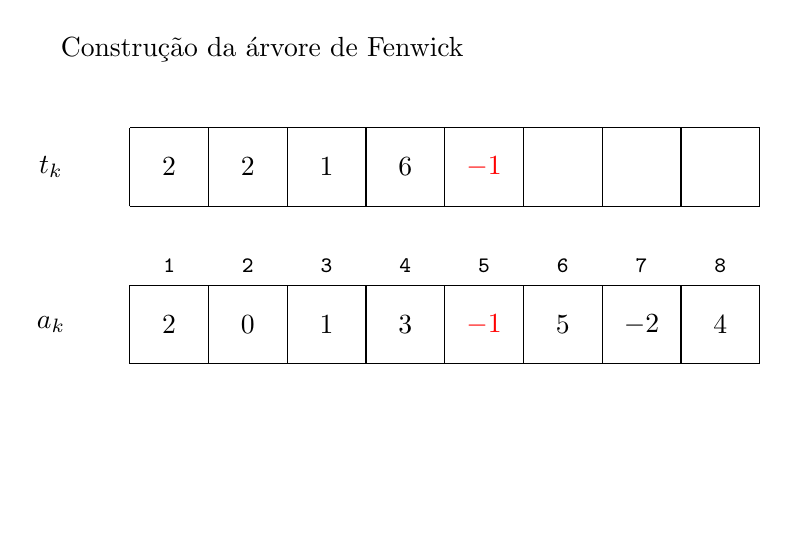
\begin{tikzpicture}
            \node[anchor=west] at (0, 12) { Construção da árvore de Fenwick };

            \draw (1, 10) grid (9, 11);
            \draw (1, 8) grid (9, 9);

            \node at (0, 8.5) { $a_k$ };
            \node at (0, 10.5) { $t_k$ };

            \node[opacity=0, anchor=west] at (0, 6.5) { $RSQ(3,7) = RSQ(1, 7) - RSQ(1, 2)$ };

            \node at (1.5, 9.25) { \footnotesize \tt 1 };
            \node at (2.5, 9.25) { \footnotesize \tt 2 };
            \node at (3.5, 9.25) { \footnotesize \tt 3 };
            \node at (4.5, 9.25) { \footnotesize \tt 4 };
            \node at (5.5, 9.25) { \footnotesize \tt 5 };
            \node at (6.5, 9.25) { \footnotesize \tt 6 };
            \node at (7.5, 9.25) { \footnotesize \tt 7 };
            \node at (8.5, 9.25) { \footnotesize \tt 8 };

            \node at (1.5, 8.5) { \textcolor{black}{$2$} };
            \node at (2.5, 8.5) { \textcolor{black}{$0$} };
            \node at (3.5, 8.5) { \textcolor{black}{$1$} };
            \node at (4.5, 8.5) { \textcolor{black}{$3$} };
            \node at (5.5, 8.5) { \textcolor{red}{$-1$} };
            \node at (6.5, 8.5) { $5$ };
            \node at (7.5, 8.5) { $-2$ };
            \node at (8.5, 8.5) { $4$ };

            \node at (1.5, 10.5) { \textcolor{black}{$2$} };
            \node at (2.5, 10.5) { \textcolor{black}{$2$} };
            \node at (3.5, 10.5) { \textcolor{black}{$1$} };
            \node at (4.5, 10.5) { \textcolor{black}{$6$} };
            \node at (5.5, 10.5) { \textcolor{red}{$-1$} };

        \end{tikzpicture}

    \end{figure}

\end{frame}

\begin{frame}[fragile]{Visualização de uma RSQ em uma BITree}

    \begin{figure}
        \centering

        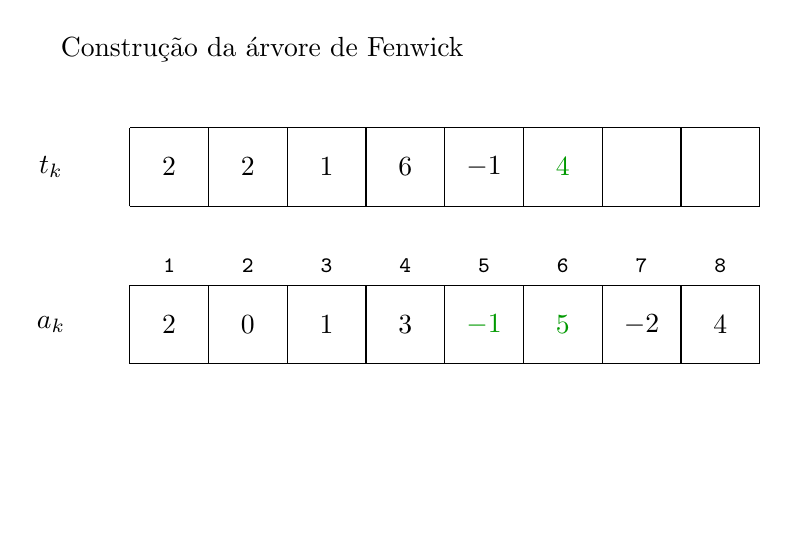
\begin{tikzpicture}
            \node[anchor=west] at (0, 12) { Construção da árvore de Fenwick };

            \draw (1, 10) grid (9, 11);
            \draw (1, 8) grid (9, 9);

            \node at (0, 8.5) { $a_k$ };
            \node at (0, 10.5) { $t_k$ };

            \node[opacity=0, anchor=west] at (0, 6.5) { $RSQ(3,7) = RSQ(1, 7) - RSQ(1, 2)$ };

            \node at (1.5, 9.25) { \footnotesize \tt 1 };
            \node at (2.5, 9.25) { \footnotesize \tt 2 };
            \node at (3.5, 9.25) { \footnotesize \tt 3 };
            \node at (4.5, 9.25) { \footnotesize \tt 4 };
            \node at (5.5, 9.25) { \footnotesize \tt 5 };
            \node at (6.5, 9.25) { \footnotesize \tt 6 };
            \node at (7.5, 9.25) { \footnotesize \tt 7 };
            \node at (8.5, 9.25) { \footnotesize \tt 8 };

            \node at (1.5, 8.5) { \textcolor{black}{$2$} };
            \node at (2.5, 8.5) { \textcolor{black}{$0$} };
            \node at (3.5, 8.5) { \textcolor{black}{$1$} };
            \node at (4.5, 8.5) { \textcolor{black}{$3$} };
            \node at (5.5, 8.5) { \textcolor{green!60!black}{$-1$} };
            \node at (6.5, 8.5) { \textcolor{green!60!black}{$5$} };
            \node at (7.5, 8.5) { $-2$ };
            \node at (8.5, 8.5) { $4$ };

            \node at (1.5, 10.5) { \textcolor{black}{$2$} };
            \node at (2.5, 10.5) { \textcolor{black}{$2$} };
            \node at (3.5, 10.5) { \textcolor{black}{$1$} };
            \node at (4.5, 10.5) { \textcolor{black}{$6$} };
            \node at (5.5, 10.5) { \textcolor{black}{$-1$} };
            \node at (6.5, 10.5) { \textcolor{green!60!black}{$4$} };

        \end{tikzpicture}

    \end{figure}

\end{frame}

\begin{frame}[fragile]{Visualização de uma RSQ em uma BITree}

    \begin{figure}
        \centering

        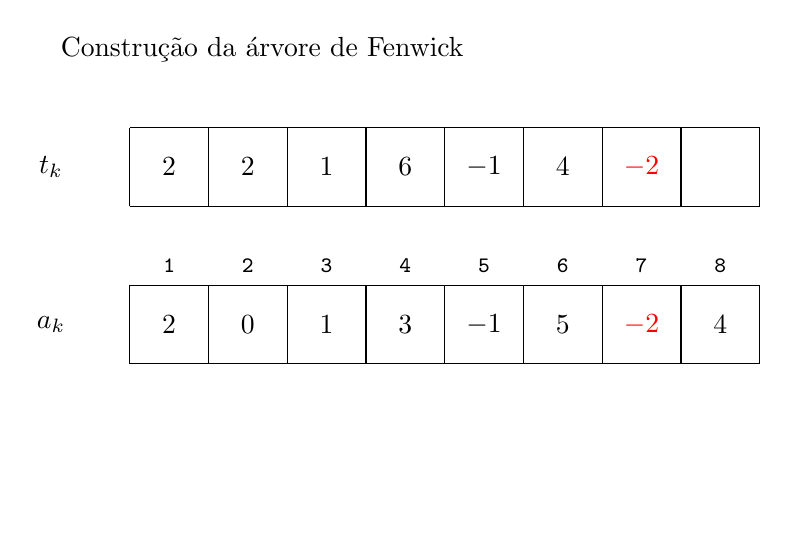
\begin{tikzpicture}
            \node[anchor=west] at (0, 12) { Construção da árvore de Fenwick };

            \draw (1, 10) grid (9, 11);
            \draw (1, 8) grid (9, 9);

            \node at (0, 8.5) { $a_k$ };
            \node at (0, 10.5) { $t_k$ };

            \node[opacity=0, anchor=west] at (0, 6.5) { $RSQ(3,7) = RSQ(1, 7) - RSQ(1, 2)$ };

            \node at (1.5, 9.25) { \footnotesize \tt 1 };
            \node at (2.5, 9.25) { \footnotesize \tt 2 };
            \node at (3.5, 9.25) { \footnotesize \tt 3 };
            \node at (4.5, 9.25) { \footnotesize \tt 4 };
            \node at (5.5, 9.25) { \footnotesize \tt 5 };
            \node at (6.5, 9.25) { \footnotesize \tt 6 };
            \node at (7.5, 9.25) { \footnotesize \tt 7 };
            \node at (8.5, 9.25) { \footnotesize \tt 8 };

            \node at (1.5, 8.5) { \textcolor{black}{$2$} };
            \node at (2.5, 8.5) { \textcolor{black}{$0$} };
            \node at (3.5, 8.5) { \textcolor{black}{$1$} };
            \node at (4.5, 8.5) { \textcolor{black}{$3$} };
            \node at (5.5, 8.5) { \textcolor{black}{$-1$} };
            \node at (6.5, 8.5) { \textcolor{black}{$5$} };
            \node at (7.5, 8.5) { \textcolor{red}{$-2$} };
            \node at (8.5, 8.5) { $4$ };

            \node at (1.5, 10.5) { \textcolor{black}{$2$} };
            \node at (2.5, 10.5) { \textcolor{black}{$2$} };
            \node at (3.5, 10.5) { \textcolor{black}{$1$} };
            \node at (4.5, 10.5) { \textcolor{black}{$6$} };
            \node at (5.5, 10.5) { \textcolor{black}{$-1$} };
            \node at (6.5, 10.5) { \textcolor{black}{$4$} };
            \node at (7.5, 10.5) { \textcolor{red}{$-2$} };

        \end{tikzpicture}

    \end{figure}

\end{frame}

\begin{frame}[fragile]{Visualização de uma RSQ em uma BITree}

    \begin{figure}
        \centering

        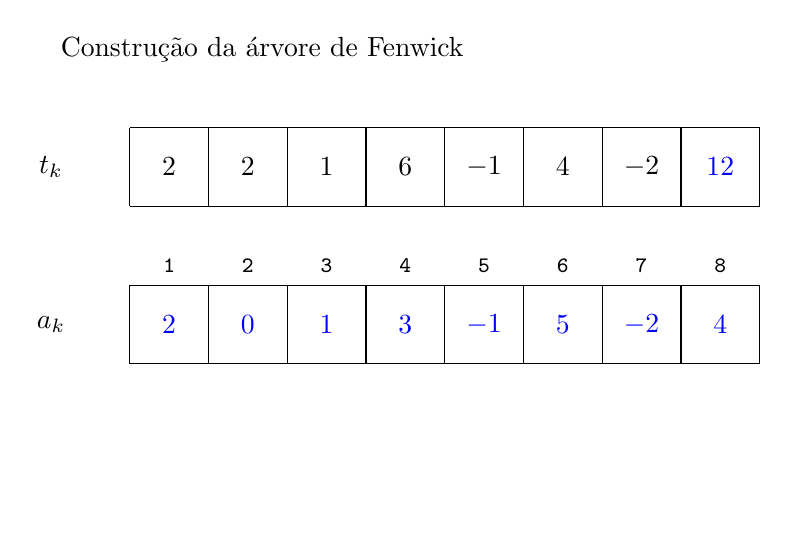
\begin{tikzpicture}
            \node[anchor=west] at (0, 12) { Construção da árvore de Fenwick };

            \draw (1, 10) grid (9, 11);
            \draw (1, 8) grid (9, 9);

            \node at (0, 8.5) { $a_k$ };
            \node at (0, 10.5) { $t_k$ };

            \node[opacity=0, anchor=west] at (0, 6.5) { $RSQ(3,7) = RSQ(1, 7) - RSQ(1, 2)$ };

            \node at (1.5, 9.25) { \footnotesize \tt 1 };
            \node at (2.5, 9.25) { \footnotesize \tt 2 };
            \node at (3.5, 9.25) { \footnotesize \tt 3 };
            \node at (4.5, 9.25) { \footnotesize \tt 4 };
            \node at (5.5, 9.25) { \footnotesize \tt 5 };
            \node at (6.5, 9.25) { \footnotesize \tt 6 };
            \node at (7.5, 9.25) { \footnotesize \tt 7 };
            \node at (8.5, 9.25) { \footnotesize \tt 8 };

            \node at (1.5, 8.5) { \textcolor{blue}{$2$} };
            \node at (2.5, 8.5) { \textcolor{blue}{$0$} };
            \node at (3.5, 8.5) { \textcolor{blue}{$1$} };
            \node at (4.5, 8.5) { \textcolor{blue}{$3$} };
            \node at (5.5, 8.5) { \textcolor{blue}{$-1$} };
            \node at (6.5, 8.5) { \textcolor{blue}{$5$} };
            \node at (7.5, 8.5) { \textcolor{blue}{$-2$} };
            \node at (8.5, 8.5) { \textcolor{blue}{$4$} };

            \node at (1.5, 10.5) { \textcolor{black}{$2$} };
            \node at (2.5, 10.5) { \textcolor{black}{$2$} };
            \node at (3.5, 10.5) { \textcolor{black}{$1$} };
            \node at (4.5, 10.5) { \textcolor{black}{$6$} };
            \node at (5.5, 10.5) { \textcolor{black}{$-1$} };
            \node at (6.5, 10.5) { \textcolor{black}{$4$} };
            \node at (7.5, 10.5) { \textcolor{black}{$-2$} };
            \node at (8.5, 10.5) { \textcolor{blue}{$12$} };

        \end{tikzpicture}

    \end{figure}

\end{frame}

\begin{frame}[fragile]{Visualização de uma RSQ em uma BITree}

    \begin{figure}
        \centering

        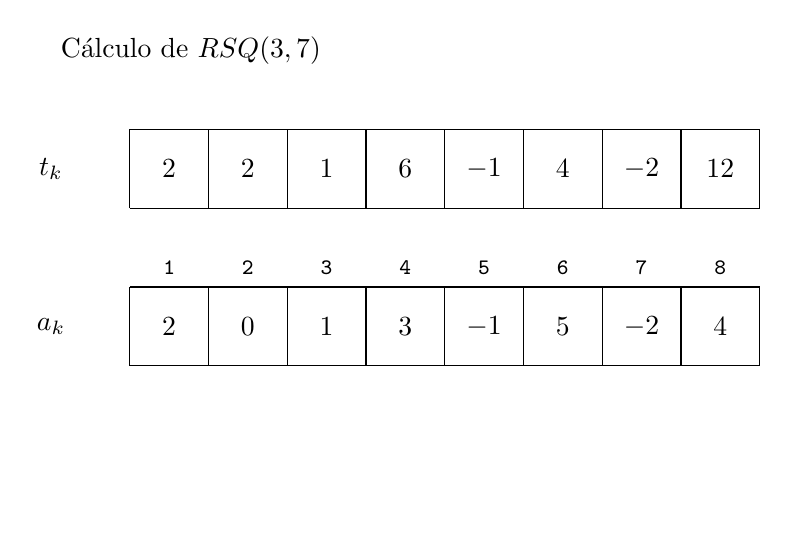
\begin{tikzpicture}
            \node[anchor=west] at (0, 12) { Cálculo de $RSQ(3, 7)$ };

            \draw (1, 10) grid (9, 11);
            \draw (1, 8) grid (9, 9);

            \node at (0, 8.5) { $a_k$ };
            \node at (0, 10.5) { $t_k$ };

            \node[opacity=0, anchor=west] at (0, 6.5) { $RSQ(3,7) = RSQ(1, 7) - RSQ(1, 2)$ };

            \node at (1.5, 9.25) { \footnotesize \tt 1 };
            \node at (2.5, 9.25) { \footnotesize \tt 2 };
            \node at (3.5, 9.25) { \footnotesize \tt 3 };
            \node at (4.5, 9.25) { \footnotesize \tt 4 };
            \node at (5.5, 9.25) { \footnotesize \tt 5 };
            \node at (6.5, 9.25) { \footnotesize \tt 6 };
            \node at (7.5, 9.25) { \footnotesize \tt 7 };
            \node at (8.5, 9.25) { \footnotesize \tt 8 };

            \node at (1.5, 8.5) { \textcolor{black}{$2$} };
            \node at (2.5, 8.5) { \textcolor{black}{$0$} };
            \node at (3.5, 8.5) { \textcolor{black}{$1$} };
            \node at (4.5, 8.5) { \textcolor{black}{$3$} };
            \node at (5.5, 8.5) { \textcolor{black}{$-1$} };
            \node at (6.5, 8.5) { \textcolor{black}{$5$} };
            \node at (7.5, 8.5) { \textcolor{black}{$-2$} };
            \node at (8.5, 8.5) { \textcolor{black}{$4$} };

            \node at (1.5, 10.5) { \textcolor{black}{$2$} };
            \node at (2.5, 10.5) { \textcolor{black}{$2$} };
            \node at (3.5, 10.5) { \textcolor{black}{$1$} };
            \node at (4.5, 10.5) { \textcolor{black}{$6$} };
            \node at (5.5, 10.5) { \textcolor{black}{$-1$} };
            \node at (6.5, 10.5) { \textcolor{black}{$4$} };
            \node at (7.5, 10.5) { \textcolor{black}{$-2$} };
            \node at (8.5, 10.5) { \textcolor{black}{$12$} };

        \end{tikzpicture}

    \end{figure}

\end{frame}

\begin{frame}[fragile]{Visualização de uma RSQ em uma BITree}

    \begin{figure}
        \centering

        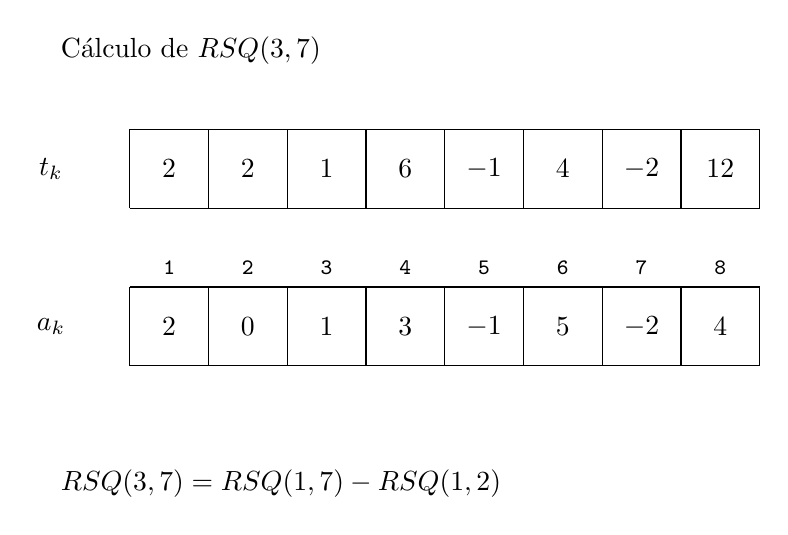
\begin{tikzpicture}
            \node[anchor=west] at (0, 12) { Cálculo de $RSQ(3, 7)$ };

            \draw (1, 10) grid (9, 11);
            \draw (1, 8) grid (9, 9);

            \node at (0, 8.5) { $a_k$ };
            \node at (0, 10.5) { $t_k$ };

            \node[anchor=west] at (0, 6.5) { $RSQ(3,7) = RSQ(1, 7) - RSQ(1, 2)$ };

            \node at (1.5, 9.25) { \footnotesize \tt 1 };
            \node at (2.5, 9.25) { \footnotesize \tt 2 };
            \node at (3.5, 9.25) { \footnotesize \tt 3 };
            \node at (4.5, 9.25) { \footnotesize \tt 4 };
            \node at (5.5, 9.25) { \footnotesize \tt 5 };
            \node at (6.5, 9.25) { \footnotesize \tt 6 };
            \node at (7.5, 9.25) { \footnotesize \tt 7 };
            \node at (8.5, 9.25) { \footnotesize \tt 8 };

            \node at (1.5, 8.5) { \textcolor{black}{$2$} };
            \node at (2.5, 8.5) { \textcolor{black}{$0$} };
            \node at (3.5, 8.5) { \textcolor{black}{$1$} };
            \node at (4.5, 8.5) { \textcolor{black}{$3$} };
            \node at (5.5, 8.5) { \textcolor{black}{$-1$} };
            \node at (6.5, 8.5) { \textcolor{black}{$5$} };
            \node at (7.5, 8.5) { \textcolor{black}{$-2$} };
            \node at (8.5, 8.5) { \textcolor{black}{$4$} };

            \node at (1.5, 10.5) { \textcolor{black}{$2$} };
            \node at (2.5, 10.5) { \textcolor{black}{$2$} };
            \node at (3.5, 10.5) { \textcolor{black}{$1$} };
            \node at (4.5, 10.5) { \textcolor{black}{$6$} };
            \node at (5.5, 10.5) { \textcolor{black}{$-1$} };
            \node at (6.5, 10.5) { \textcolor{black}{$4$} };
            \node at (7.5, 10.5) { \textcolor{black}{$-2$} };
            \node at (8.5, 10.5) { \textcolor{black}{$12$} };

        \end{tikzpicture}

    \end{figure}

\end{frame}

\begin{frame}[fragile]{Visualização de uma RSQ em uma BITree}

    \begin{figure}
        \centering

        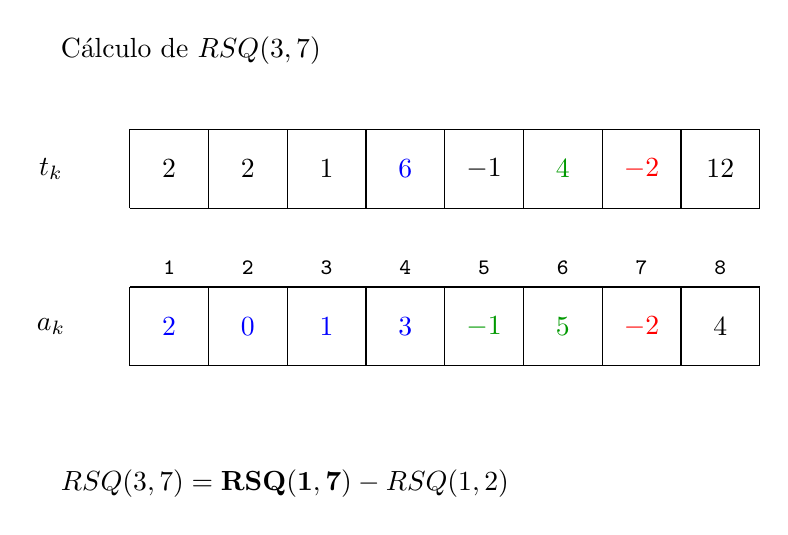
\begin{tikzpicture}
            \node[anchor=west] at (0, 12) { Cálculo de $RSQ(3, 7)$ };

            \draw (1, 10) grid (9, 11);
            \draw (1, 8) grid (9, 9);

            \node at (0, 8.5) { $a_k$ };
            \node at (0, 10.5) { $t_k$ };

            \node[anchor=west] at (0, 6.5) { $RSQ(3,7) = \mathbf{RSQ(1, 7)} - RSQ(1, 2)$ };

            \node at (1.5, 9.25) { \footnotesize \tt 1 };
            \node at (2.5, 9.25) { \footnotesize \tt 2 };
            \node at (3.5, 9.25) { \footnotesize \tt 3 };
            \node at (4.5, 9.25) { \footnotesize \tt 4 };
            \node at (5.5, 9.25) { \footnotesize \tt 5 };
            \node at (6.5, 9.25) { \footnotesize \tt 6 };
            \node at (7.5, 9.25) { \footnotesize \tt 7 };
            \node at (8.5, 9.25) { \footnotesize \tt 8 };

            \node at (1.5, 8.5) { \textcolor{blue}{$2$} };
            \node at (2.5, 8.5) { \textcolor{blue}{$0$} };
            \node at (3.5, 8.5) { \textcolor{blue}{$1$} };
            \node at (4.5, 8.5) { \textcolor{blue}{$3$} };
            \node at (5.5, 8.5) { \textcolor{green!60!black}{$-1$} };
            \node at (6.5, 8.5) { \textcolor{green!60!black}{$5$} };
            \node at (7.5, 8.5) { \textcolor{red}{$-2$} };
            \node at (8.5, 8.5) { \textcolor{black}{$4$} };

            \node at (1.5, 10.5) { \textcolor{black}{$2$} };
            \node at (2.5, 10.5) { \textcolor{black}{$2$} };
            \node at (3.5, 10.5) { \textcolor{black}{$1$} };
            \node at (4.5, 10.5) { \textcolor{blue}{$6$} };
            \node at (5.5, 10.5) { \textcolor{black}{$-1$} };
            \node at (6.5, 10.5) { \textcolor{green!60!black}{$4$} };
            \node at (7.5, 10.5) { \textcolor{red}{$-2$} };
            \node at (8.5, 10.5) { \textcolor{black}{$12$} };

        \end{tikzpicture}

    \end{figure}

\end{frame}

\begin{frame}[fragile]{Visualização de uma RSQ em uma BITree}

    \begin{figure}
        \centering

        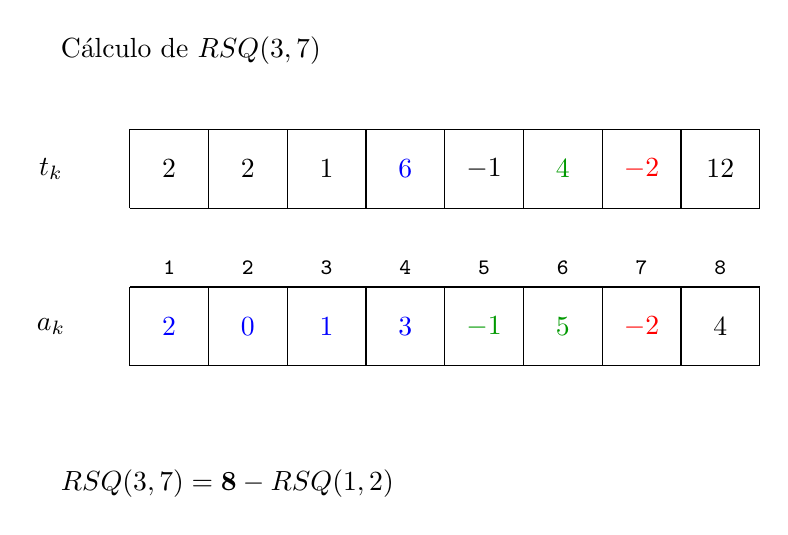
\begin{tikzpicture}
            \node[anchor=west] at (0, 12) { Cálculo de $RSQ(3, 7)$ };

            \draw (1, 10) grid (9, 11);
            \draw (1, 8) grid (9, 9);

            \node at (0, 8.5) { $a_k$ };
            \node at (0, 10.5) { $t_k$ };

            \node[anchor=west] at (0, 6.5) { $RSQ(3,7) = \mathbf{8} - RSQ(1, 2)$ };

            \node at (1.5, 9.25) { \footnotesize \tt 1 };
            \node at (2.5, 9.25) { \footnotesize \tt 2 };
            \node at (3.5, 9.25) { \footnotesize \tt 3 };
            \node at (4.5, 9.25) { \footnotesize \tt 4 };
            \node at (5.5, 9.25) { \footnotesize \tt 5 };
            \node at (6.5, 9.25) { \footnotesize \tt 6 };
            \node at (7.5, 9.25) { \footnotesize \tt 7 };
            \node at (8.5, 9.25) { \footnotesize \tt 8 };

            \node at (1.5, 8.5) { \textcolor{blue}{$2$} };
            \node at (2.5, 8.5) { \textcolor{blue}{$0$} };
            \node at (3.5, 8.5) { \textcolor{blue}{$1$} };
            \node at (4.5, 8.5) { \textcolor{blue}{$3$} };
            \node at (5.5, 8.5) { \textcolor{green!60!black}{$-1$} };
            \node at (6.5, 8.5) { \textcolor{green!60!black}{$5$} };
            \node at (7.5, 8.5) { \textcolor{red}{$-2$} };
            \node at (8.5, 8.5) { \textcolor{black}{$4$} };

            \node at (1.5, 10.5) { \textcolor{black}{$2$} };
            \node at (2.5, 10.5) { \textcolor{black}{$2$} };
            \node at (3.5, 10.5) { \textcolor{black}{$1$} };
            \node at (4.5, 10.5) { \textcolor{blue}{$6$} };
            \node at (5.5, 10.5) { \textcolor{black}{$-1$} };
            \node at (6.5, 10.5) { \textcolor{green!60!black}{$4$} };
            \node at (7.5, 10.5) { \textcolor{red}{$-2$} };
            \node at (8.5, 10.5) { \textcolor{black}{$12$} };

        \end{tikzpicture}

    \end{figure}

\end{frame}

\begin{frame}[fragile]{Visualização de uma RSQ em uma BITree}

    \begin{figure}
        \centering

        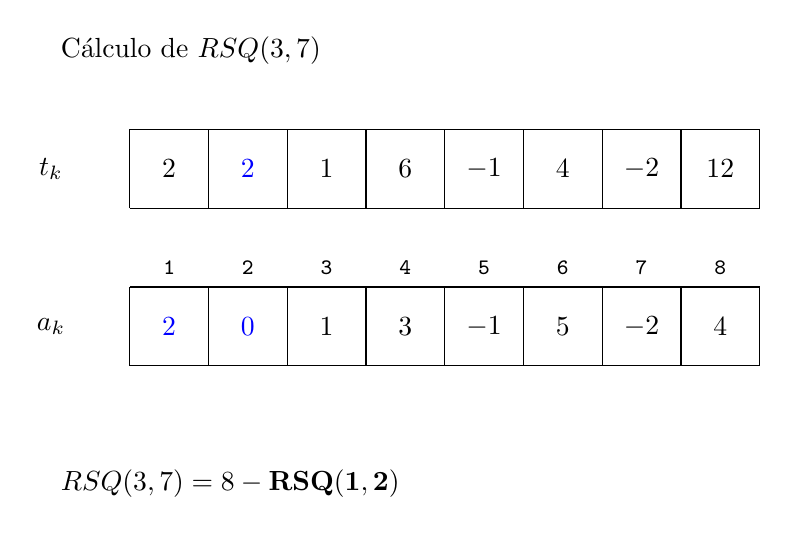
\begin{tikzpicture}
            \node[anchor=west] at (0, 12) { Cálculo de $RSQ(3, 7)$ };

            \draw (1, 10) grid (9, 11);
            \draw (1, 8) grid (9, 9);

            \node at (0, 8.5) { $a_k$ };
            \node at (0, 10.5) { $t_k$ };

            \node[anchor=west] at (0, 6.5) { $RSQ(3,7) = 8 - \mathbf{RSQ(1, 2)}$ };

            \node at (1.5, 9.25) { \footnotesize \tt 1 };
            \node at (2.5, 9.25) { \footnotesize \tt 2 };
            \node at (3.5, 9.25) { \footnotesize \tt 3 };
            \node at (4.5, 9.25) { \footnotesize \tt 4 };
            \node at (5.5, 9.25) { \footnotesize \tt 5 };
            \node at (6.5, 9.25) { \footnotesize \tt 6 };
            \node at (7.5, 9.25) { \footnotesize \tt 7 };
            \node at (8.5, 9.25) { \footnotesize \tt 8 };

            \node at (1.5, 8.5) { \textcolor{blue}{$2$} };
            \node at (2.5, 8.5) { \textcolor{blue}{$0$} };
            \node at (3.5, 8.5) { \textcolor{black}{$1$} };
            \node at (4.5, 8.5) { \textcolor{black}{$3$} };
            \node at (5.5, 8.5) { \textcolor{black}{$-1$} };
            \node at (6.5, 8.5) { \textcolor{black}{$5$} };
            \node at (7.5, 8.5) { \textcolor{black}{$-2$} };
            \node at (8.5, 8.5) { \textcolor{black}{$4$} };

            \node at (1.5, 10.5) { \textcolor{black}{$2$} };
            \node at (2.5, 10.5) { \textcolor{blue}{$2$} };
            \node at (3.5, 10.5) { \textcolor{black}{$1$} };
            \node at (4.5, 10.5) { \textcolor{black}{$6$} };
            \node at (5.5, 10.5) { \textcolor{black}{$-1$} };
            \node at (6.5, 10.5) { \textcolor{black}{$4$} };
            \node at (7.5, 10.5) { \textcolor{black}{$-2$} };
            \node at (8.5, 10.5) { \textcolor{black}{$12$} };

        \end{tikzpicture}

    \end{figure}

\end{frame}

\begin{frame}[fragile]{Visualização de uma RSQ em uma BITree}

    \begin{figure}
        \centering

        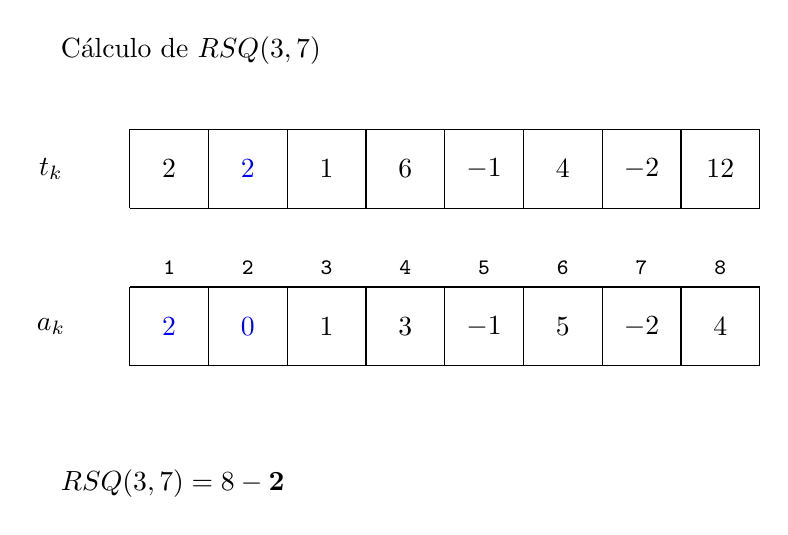
\begin{tikzpicture}
            \node[anchor=west] at (0, 12) { Cálculo de $RSQ(3, 7)$ };

            \draw (1, 10) grid (9, 11);
            \draw (1, 8) grid (9, 9);

            \node at (0, 8.5) { $a_k$ };
            \node at (0, 10.5) { $t_k$ };

            \node[anchor=west] at (0, 6.5) { $RSQ(3,7) = 8 - \mathbf{2}$ };

            \node at (1.5, 9.25) { \footnotesize \tt 1 };
            \node at (2.5, 9.25) { \footnotesize \tt 2 };
            \node at (3.5, 9.25) { \footnotesize \tt 3 };
            \node at (4.5, 9.25) { \footnotesize \tt 4 };
            \node at (5.5, 9.25) { \footnotesize \tt 5 };
            \node at (6.5, 9.25) { \footnotesize \tt 6 };
            \node at (7.5, 9.25) { \footnotesize \tt 7 };
            \node at (8.5, 9.25) { \footnotesize \tt 8 };

            \node at (1.5, 8.5) { \textcolor{blue}{$2$} };
            \node at (2.5, 8.5) { \textcolor{blue}{$0$} };
            \node at (3.5, 8.5) { \textcolor{black}{$1$} };
            \node at (4.5, 8.5) { \textcolor{black}{$3$} };
            \node at (5.5, 8.5) { \textcolor{black}{$-1$} };
            \node at (6.5, 8.5) { \textcolor{black}{$5$} };
            \node at (7.5, 8.5) { \textcolor{black}{$-2$} };
            \node at (8.5, 8.5) { \textcolor{black}{$4$} };

            \node at (1.5, 10.5) { \textcolor{black}{$2$} };
            \node at (2.5, 10.5) { \textcolor{blue}{$2$} };
            \node at (3.5, 10.5) { \textcolor{black}{$1$} };
            \node at (4.5, 10.5) { \textcolor{black}{$6$} };
            \node at (5.5, 10.5) { \textcolor{black}{$-1$} };
            \node at (6.5, 10.5) { \textcolor{black}{$4$} };
            \node at (7.5, 10.5) { \textcolor{black}{$-2$} };
            \node at (8.5, 10.5) { \textcolor{black}{$12$} };

        \end{tikzpicture}

    \end{figure}

\end{frame}

\begin{frame}[fragile]{Visualização de uma RSQ em uma BITree}

    \begin{figure}
        \centering

        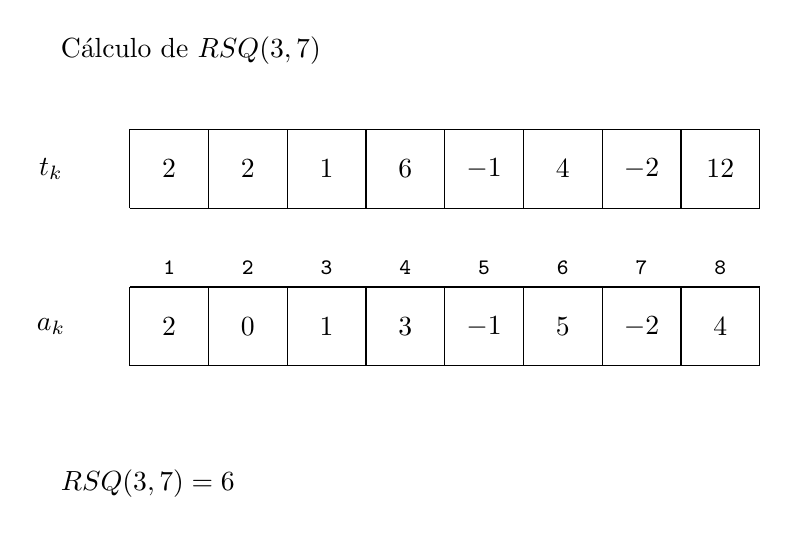
\begin{tikzpicture}
            \node[anchor=west] at (0, 12) { Cálculo de $RSQ(3, 7)$ };

            \draw (1, 10) grid (9, 11);
            \draw (1, 8) grid (9, 9);

            \node at (0, 8.5) { $a_k$ };
            \node at (0, 10.5) { $t_k$ };

            \node[anchor=west] at (0, 6.5) { $RSQ(3,7) = 6 $ };

            \node at (1.5, 9.25) { \footnotesize \tt 1 };
            \node at (2.5, 9.25) { \footnotesize \tt 2 };
            \node at (3.5, 9.25) { \footnotesize \tt 3 };
            \node at (4.5, 9.25) { \footnotesize \tt 4 };
            \node at (5.5, 9.25) { \footnotesize \tt 5 };
            \node at (6.5, 9.25) { \footnotesize \tt 6 };
            \node at (7.5, 9.25) { \footnotesize \tt 7 };
            \node at (8.5, 9.25) { \footnotesize \tt 8 };

            \node at (1.5, 8.5) { \textcolor{black}{$2$} };
            \node at (2.5, 8.5) { \textcolor{black}{$0$} };
            \node at (3.5, 8.5) { \textcolor{black}{$1$} };
            \node at (4.5, 8.5) { \textcolor{black}{$3$} };
            \node at (5.5, 8.5) { \textcolor{black}{$-1$} };
            \node at (6.5, 8.5) { \textcolor{black}{$5$} };
            \node at (7.5, 8.5) { \textcolor{black}{$-2$} };
            \node at (8.5, 8.5) { \textcolor{black}{$4$} };

            \node at (1.5, 10.5) { \textcolor{black}{$2$} };
            \node at (2.5, 10.5) { \textcolor{black}{$2$} };
            \node at (3.5, 10.5) { \textcolor{black}{$1$} };
            \node at (4.5, 10.5) { \textcolor{black}{$6$} };
            \node at (5.5, 10.5) { \textcolor{black}{$-1$} };
            \node at (6.5, 10.5) { \textcolor{black}{$4$} };
            \node at (7.5, 10.5) { \textcolor{black}{$-2$} };
            \node at (8.5, 10.5) { \textcolor{black}{$12$} };

        \end{tikzpicture}

    \end{figure}

\end{frame}
